\chapter{系统设计}

\section{数据结构设计}

对于每一条语句,我们都将生成一个自动机,它具有startNode和endNode两个state节点,并且
有一条边从startNode连到endNode,对于日志函数,边上的标签即是它的输出。
\begin{figure}[htbp]
	\centering
	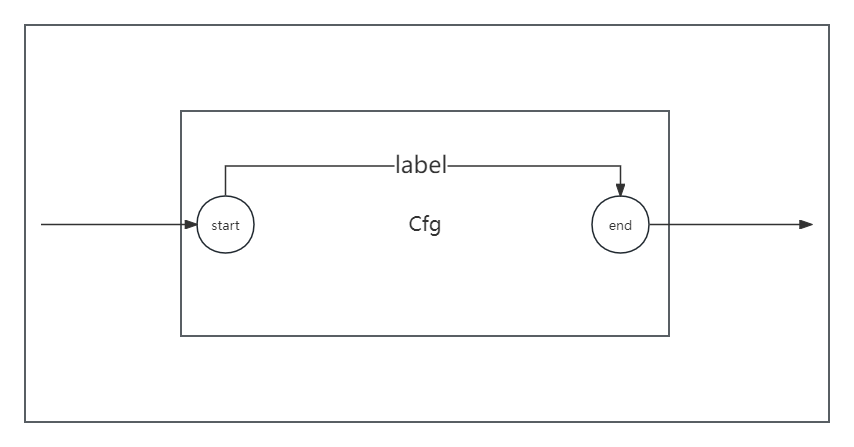
\includegraphics[width=0.5\textwidth]{pictures/Cfg.png}
	\caption{自动机的数据结构}
	\label{fig:自动机的数据结构}
\end{figure}
整个系统生成CFG的过程就是递归生成自动机,并合并自动机的过程。
state节点在系统中用astNode存储,它保存了state节点的内置id。
\begin{figure}[htbp]
	\centering
	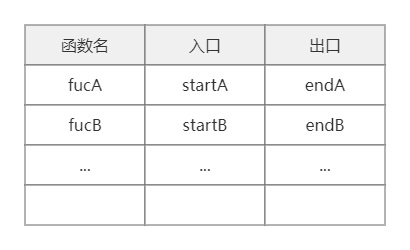
\includegraphics[width=0.5\textwidth]{pictures/fucTable.png}
	\caption{函数表}
	\label{fig:函数表}
\end{figure}
对于整个图结构,本系统采用的是networkx中的有向图来存储,同时我们也要存下自动机的字母表,用于对后续的DFA进行识别,另外,当遇到函数调用时,
为了知道入口函数的位置,我们也需要用一个函数表来通过函数的名字去查找它的入口和出口。
\section{程序流程设计}
对于本系统的主要模块,大致的流程是这样的:
\begin{enumerate}
	\item 使用clang扫描c++源文件,生成clang-AST
    \item 通过遍历AST,递归生成初始的CFG
    \item 对于CFG,获取日志函数的相关信息,生成相应的NFA
    \item 将NFA转换成为DFA
    \item 识别DFA
\end{enumerate}
\begin{figure}[htbp]
	\centering
	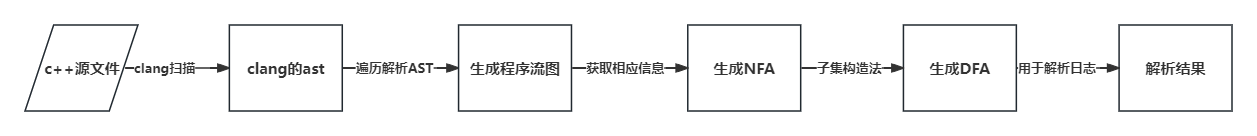
\includegraphics[width=1\textwidth]{pictures/系统流程.png}
	\caption{系统流程图}
	\label{fig:系统流程图}
\end{figure}

